\NeedsTeXFormat{LaTeX2e}[1995/12/01]
\documentclass[10pt]{bmc_article}    

\usepackage{cite} % Make references as [1-4], not [1,2,3,4]
\usepackage{url}  % Formatting web addresses  
\usepackage{ifthen}  % Conditional 
\usepackage{multicol}   %Columns
\usepackage[utf8]{inputenc} %unicode support
%\usepackage[latin1]{inputenc} %UNIX support if unicode package fails
\urlstyle{rm}
\usepackage[pdftex]{graphicx}
 
%\def\includegraphic{}
%\def\includegraphics{}

\setlength{\topmargin}{0.0cm}
\setlength{\textheight}{21.5cm}
\setlength{\oddsidemargin}{0cm} 
\setlength{\textwidth}{16.5cm}
\setlength{\columnsep}{0.6cm}

\newboolean{publ}

\newenvironment{bmcformat}{\begin{raggedright}\baselineskip20pt\sloppy\setboolean{publ}{false}}{\end{raggedright}\baselineskip20pt\sloppy}

%Publication style settings
%\newenvironment{bmcformat}{\fussy\setboolean{publ}{true}}{\fussy}

% Begin ...
\begin{document}
\begin{bmcformat}

\title{Resource Description Framework Technologies in Chemistry}
 
\author{Egon L Willighagen\correspondingauthor$^{1}$%
       \email{Egon L Willighagen\correspondingauthor - egon.willighagen@ki.se}%
       and 
         Martin P Br\"andle$^2$%
         \email{Martin P Br\"andle - braendle@chem.ethz.ch}%
      }

\address{%
    \iid(1)Division of Molecular Toxicology, Institute of Environmental Medicine, Karolinska Institutet, SE-17177 Stockholm, Sweden\\
    \iid(2)Chemistry Biology Pharmacy Information Center, ETH Z\"urich, Wolfgang-Pauli-Str. 10, 8093 Z\"urich, Switzerland
}%

\maketitle


%\begin{abstract}
%        \paragraph*{Background:} Text for this section of the abstract. 
%        \paragraph*{Results:} Text for this section of the abstract \ldots
%        \paragraph*{Conclusions:} Text for this section of the abstract \ldots
%\end{abstract}

% I don't think an abstract is required for an Editorial/mb

The Resource Description Framework (RDF) is providing the life sciences with new standards
around data and knowledge management. The uptake in the life sciences is
significantly higher than the uptake of the eXtensible Markup Language (XML)
and even relational databases, as was recently shown by Splendiani et
al.~\cite{Splendiani2011}. Chemistry is adopting these methods too.
For example, Murray-Rust and coworkers used RDF already in 2004 to distribute
news items where chemical structures were embedded using RDF Site Summary 1.0.~\cite{MurrayRust2004}
Frey implemented a system which would now be referred to an
electronic lab notebook (ELN).~\cite{Frey2004} The use of the SPARQL
query language goes back to 2007 where it was used in a system to annotate
crystal structures.~\cite{Hunter2007}

The American Chemical Society (ACS) Division of Chemical Information (CINF)
invited scientists from around the world to present their use of RDF
technologies in chemistry on 22nd-23rd August 2010
at the 240th ACS National Meeting in Boston, USA. During three half-day
sessions, the speakers demonstrated a mix of smaller and larger initiatives
where RDF and related technologies are used in cheminformatics and
bioinformatics as Open Standards for data exchange, common languages
(ontologies), and problem solving. The fifteen presentations were grouped in the themes computation,
ontologies, and chemical applications. Figures~1 to~3 display the most important
keywords reflecting the abstracts of the talks in each session as word
clouds~\cite{WORDLE}.

The goal of the meeting was to make more chemists aware of what the RDF Open
Standard has to offer to chemistry. We are delighted to continue this effort
with this thematic issue, for which the speakers (and others) were invited
to present their work in more detail to a wider chemistry community. The choice
of an Open Access journal follows this goal. At this place, we would like to thank Pfizer, Inc., 
who had partially funded the article processing charges for this Thematic Series.
Pfizer, Inc. has had no input into the content of the publication or the articles themselves.
All articles in the series were independently prepared by the authors and
were subjected to the journal's standard peer review process.

In the remainder of this editorial, we will briefly outline the various RDF
technologies and how they have been used in chemistry so far.

\section{Concepts}

The core RDF specification was introduced by the World Wide Web Consortium (W3C)
in 1999~\cite{Lassila1999} and defines the foundation of the RDF technologies. It has
evolved into a set of six recommendations by W3C published in 2004
(See Table~1). 
RDF specifies a very simple data structure linking a subject to an object or a
value (literal) using a predicate. Cheminformaticians will recognize this data
structure as an edge from graph theory. This structure allows us to represent
facts like ``vanillin dissolves in methyl alcohol''~\cite{ONS2010}. RDF uses Uniform
Resource Identifiers (URIs) to identify things. Therefore, the RDF equivalent of
the solution statement could be like this so-called triple:

http://dbpedia.org/resource/Vanillin http://example.com/dissolvesIn http://dbpedia.org/resource/Methanol .

Since URIs may be used to reference resources on any server worldwide,
RDF triples allow to span a global graph data structure. 
This is not surprising, since RDF is the core technology behind the
proposed Semantic Web~\cite{BER2001}. In fact, the Web
nature is clear here, as one can follow both the URIs for vanillin and methanol to
obtain further information on those two chemicals. These molecules' URIs are said to be
dereferencable, allowing agents to spider the Web for information following
the hyperlinks, quite like how you follow hyperlinks on websites. Hence, the term Semantic Web.

Recent projects such as Bio2RDF~\cite{BEL2008}, Chem2Bio2RDF~\cite{CHE2010},
and OpenTox~\cite{Hardy2010} have brought genomic, pharmaceutical and
chemical knowledge to the Semantic Web by expressing it in RDF.
These three projects aim at making databases with chemical knowledge
available from a central access point, interlinking the individual
data sets. Smaller data sets are also becoming available as RDF, such as
the Open Notebook Science Solubility data~\cite{citeulike:5441072}. 

\section{Formats}

The actual use of RDF depends on various further standards. For example, standards were required
that describe how RDF statements are exchanged. Several standards
serve this purpose: RDF/XML is an XML-based serialization~\cite{Beckett2004}, while
easier formats exist with N-Triples~\cite{Beckett2004b} and Notation3.~\cite{BernersLee2006} For integration with
current web practices, RDFa has been defined to allow RDF triples to be embedded
in HTML pages.~\cite{RDFA2008} Additionally, a proposal has been written that
describe how RDF can be serialized as Javascript Object Notation (JSON)~\cite{Alexander2008}, and
while this is not a formal specification yet,
a new RDF working group will formalize this into a new standards.~\cite{Herman2010} Several
of these serialization standards are used in the papers in this Series.

Using these serializations, RDF can be downloaded directly from pure RDF
documents (RDF/XML, Notation3), or extracted from RDFa-based web pages using
online RDF extraction web services, like http://www.w3.org/2007/08/pyRdfa/.
These approaches make it simple to aggregate chemical data from web pages.

\section{Querying the World Wide Web}

The most promising technology in the RDF family is the
SPARQL Query Language (SPARQL)~\cite{PrudHommeaux2008}, which has been
applied by Chen et al. in three chemogenomics use cases.~\cite{CHE2010}
One of the use cases shows how SPARQL queries are used to find compounds 
that are active in bioassay for genes related to proteins
to which the chemical dexamethasone binds, using information
from PubChem, Uniprot, and DrugBank, all made available as RDF in the Chem2Bio2RDF
database. The other use cases in this paper use the same approach
by aggregating data sources before querying them. As such, it is similar to
querying data stored in a relational database. One difference between SPARQL
engines and relational databases is that the former can be run on any
RDF resource regardless of their data structure.

For example, Jankowski used a public
SPARQL service to extract boiling points of a series of alkanes from an XHTML
webpage with the data made machine readable with RDFa, and visualized that using
Javascript in another web page dynamically~\cite{Jankowski2010} (see
Figure~4). A second important difference is that SPARQL queries can be
\textit{federated}.~\cite{Prudhommeaux2007}
Federated SPARQL allows one to query various RDF providers in one query. This has
been used recently in the Receptor Explorer tool to help translational research
by connecting basic neuroscience research with clinical trials~\cite{Cheung2009}.
Being able to query resources in this manner, brings us a step closer to
systems biology approaches.

\section{Ontologies}

With RDF we have a data structure to link resources and provide details about
those resources, and SPARQL provides us with the tools to query and aggregate that data.
The next standard we will discuss now is the Web Ontology
Language (OWL) which brought the RDF technology to the ontology community~\cite{GUN2004}.
Ontologies are most certainly not new to chemistry~\cite{Gordon1988} nor biology or life sciences,
but the OWL standard makes it much easier to use ontologies, partly because
they are formulated in RDF themselves. Ontologies, like
controlled vocabularies and thesauri, describe what things mean, by linking
terms to a human-readable definition. As such, ontologies are used for sharing
knowledge in a common language, as well as to organize that knowledge.
While linking resources is not new either, expressing the content of resources
in explicit terms makes it more insightful steps are undertaken, and possible
where sources of error are. For example, Konyk et al. have used OWL to link PubChem,
DrugBank, and DBPedia, noting that it offers new ways to
discover knowledge~\cite{Konyk2008}.

There are currently not many ontologies in chemistry, but many OBO Foundry-based
ontologies can be reused using an OBO to OWL mapping.~\cite{Moreira2007} This makes
available chemical ontologies like the CO ontology~\cite{Feldman2005},
the ontology of Chemical Entities of Biological Interest (ChEBI)~\cite{Degtyarenko2008,Hull2008},
and the Cheminformatics Ontology (\url{http://code.google.com/p/semanticchemistry/}),
but also other ontologies in the life sciences, such as the Gene Ontology.~\cite{Aranguren2007}
This way, OWL provides a universal standard to link data sources in life
sciences, transcending traditionally boundaries between the various domains.

The current state is that different RDF resources are using different ontologies.
This does not necessarily have to be a problem, because the ontologies can be
explicitly mapped to each other. This way, equivalent terms from two ontologies
can be formally defined as equivalent, using the OWL predicates owl:equivalentClass
and owl:equivalentProperty for classes, and owl:sameAs for instances.
Making the equivalence explicit this way improves the provenance of data integration efforts. 

\section{Outlook}

This Thematic Series shows the current state of the use of RDF in
chemistry, as presented at the ACS RDF 2010 meeting in Boston, and provides an
insight into the progress of these methods. Much of the research is currently explorative,
rather than formative, though standards are being proposed. 
It may very well turn out that some aspects of chemistry will never be expressed
in RDF, and some computation will be done without ontology-based reasoning. It is important
to realize here where RDF is positioned, namely for linking resources.
Not all chemical data are resources, and we should not want to represent
all data as resources.
Because of the use of URIs, it is very verbose relative to other formats.
There is no need to format already well-formalized data structures into
RDF, such as the various uses of matrices in computational chemistry as
RDF triples. In fact, several papers in this series outline how to
combine knowledge expressed with RDF with computational services.

The future of the use of RDF as open standards in chemistry looks
bright, and fills the needs in chemistry for semantically linking
chemical data to other data sources. RDF technologies provide a
domain-independent way for representing knowledge and its open
nature assures many alternative approaches for making data available
as RDF.

\ifthenelse{\boolean{publ}}{\begin{multicols}{2}}{}


{\ifthenelse{\boolean{publ}}{\footnotesize}{\small}
 \bibliographystyle{bmc_article}  % Style BST file
  \bibliography{editorial} }     % Bibliography file (usually '*.bib' ) 

%%%%%%%%%%%

\ifthenelse{\boolean{publ}}{\end{multicols}}{}

\clearpage

\section*{Figures}

  \subsection*{Figure 1 - Keyword cloud for the \textit{RDF and Computation} session.}
  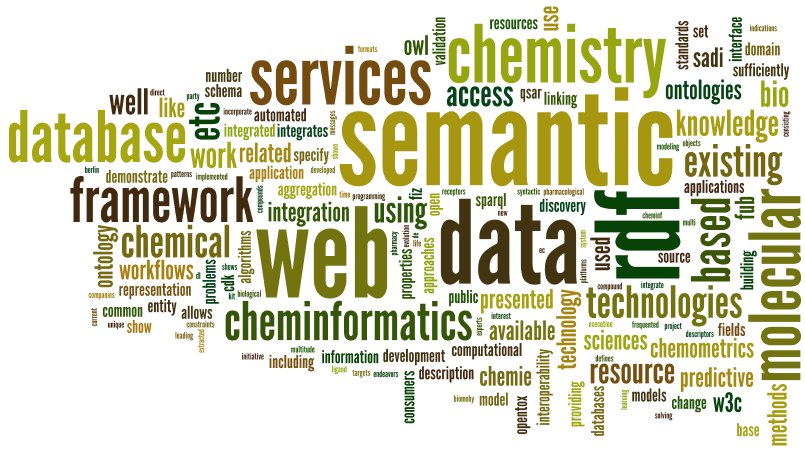
\includegraphics[width=0.5\textwidth]{graphics/wordle_cinf003} 

  \subsection*{Figure 2 - Keyword cloud for the \textit{RDF and Ontologies} session.}
  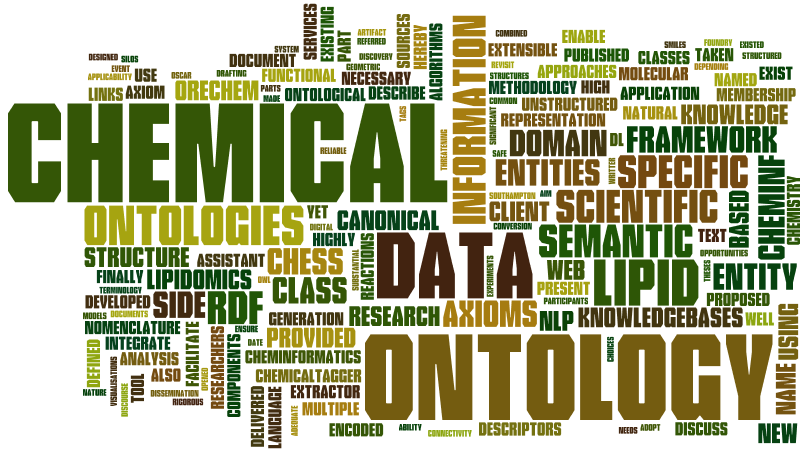
\includegraphics[width=0.5\textwidth]{graphics/wordle_cinf0031} 

  \subsection*{Figure 3 - Keyword cloud for the \textit{RDF and Chemical Applications} session.}
  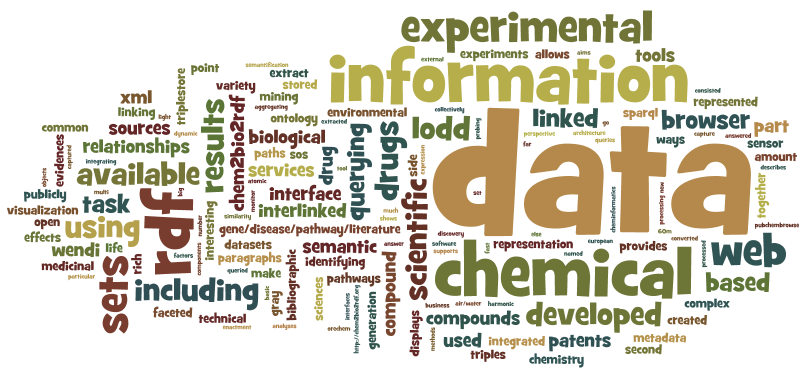
\includegraphics[width=0.5\textwidth]{graphics/wordle_cinf0032} 

  \subsection*{Figure 4 - Web page using SPARQL to visualize alkane boiling points extraced
    from another web page.}
  Web page with JavaScript by Jankowski visualizing the boiling point of a series of
  alkanes from Wiener~\cite{Wiener1947} extracted with SPARQL from a second, XHTML+RDFa web page at
  \url{http://egonw.github.com/cheminformatics.classics/classic1.html}.
  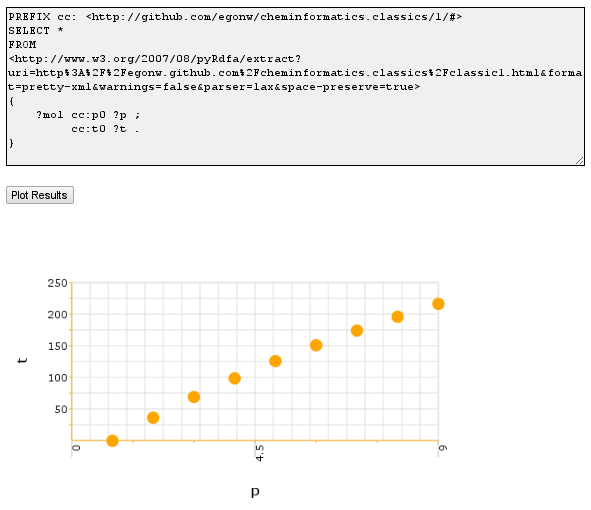
\includegraphics[width=0.7\textwidth]{graphics/sparqlGraphing1} 

\clearpage

\section*{Tables}
  \subsection*{Table 1 - Key W3C Specifications}
    Several of the key specifications and when they were
    recommended by the World Wide Web Consortium. \par \mbox{}
    \par
    \mbox{
      \begin{tabular}{lll}
        Year & Technology & Description \\ 
        \hline
        1999 & RDF     & Resource Description Framework (RDF) Model and Syntax Specification~\cite{Lassila1999} \\
        2004 & RDF/XML & RDF/XML Syntax Specification (Revised)~\cite{Beckett2004} \\
             & RDF     & Resource Description Framework (RDF): Concepts and Abstract Syntax~\cite{Carroll2004}  \\
             & OWL     & OWL Web Ontology Language Overview~\cite{OWL22009}\\
        2007 & OWL2    & OWL 2 Web Ontology Language Document Overview~\cite{OWL22009}  \\
        2008 & RDFa    & RDFa in XHTML: Syntax and Processing~\cite{RDFA2008} \\
             & SPARQL  & SPARQL Query Language for RDF~\cite{PrudHommeaux2008} \\
      \end{tabular}
      }


\end{bmcformat}
\end{document}







